\documentclass[12pt,a4paper,austrian]{article}
\usepackage{graphicx}
\usepackage[austrian, english]{babel}
\usepackage[utf8]{inputenc}
%\usepackage{listings}
\usepackage{multirow}
\usepackage{epstopdf}
\usepackage{amsmath}
\usepackage{amssymb} % fuer Mengen \N, Q, C, R
\usepackage{matlab-prettifier}
\graphicspath{{./fig/}}

\usepackage[colorlinks=true, pdfborder={0 0 0}, linkcolor=red]{hyperref}
\usepackage{float}


%% Satzspiegel
\setlength{\hoffset}{-1in} \setlength{\textwidth}{18cm}
\setlength{\oddsidemargin}{1.5cm}
\setlength{\evensidemargin}{1.5cm}
\setlength{\marginparsep}{0.7em}
\setlength{\marginparwidth}{0.5cm}

\setlength{\voffset}{-1.9in}
\setlength{\headheight}{12pt}
\setlength{\topmargin}{2.6cm}
   \addtolength{\topmargin}{-\headheight}
\setlength{\headsep}{3.5cm}
   \addtolength{\headsep}{-\topmargin}
   \addtolength{\headsep}{-\headheight}
\setlength{\textheight}{27cm}

%% How should floats be treated?
\setlength{\floatsep}{12 pt plus 0 pt minus 8 pt}
\setlength{\textfloatsep}{12 pt plus 0pt minus 8 pt}
\setlength{\intextsep}{12 pt plus 0pt minus 8 pt}

\tolerance2000
\emergencystretch20pt

%% Text appearence
% English text
\newcommand{\eg}[1]%
  {\selectlanguage{english}\textit{#1}\selectlanguage{austrian}}

\newcommand{\filename}[1]
  {\begin{small}\texttt{#1}\end{small}}

\newcommand\IFT{\unitlength1mm\begin{picture}(10,2) \put (1,1)
{\circle{1.7}} \put(2,1){\line(1,0){5}} \put(8,1)
{\circle*{1.7}}\end{picture}}
\newcommand\FT{\unitlength1mm\begin{picture}(10,2) \put (1,1)
{\circle*{1.7}} \put(2,1){\line(1,0){5}} \put(8,1)
{\circle{1.7}}\end{picture}}

% A box for multiple choice problems
\newcommand{\choicebox}{\fbox{\rule{0pt}{0.5ex}\rule{0.5ex}{0pt}}}

\newenvironment{wahrfalsch}%
  {\bigskip\par\noindent\makebox[1cm][c]{richtig}\hspace{3mm}\makebox[1cm][c]{falsch}
   \begin{list}%
   {\makebox[1cm][c]{\choicebox}\hspace{3mm}\makebox[1cm][c]{\choicebox}}%
   {\setlength{\labelwidth}{2.31 cm}\setlength{\labelsep}{3mm}
    \setlength{\leftmargin}{2.61 cm}\setlength{\listparindent}{0pt}
    \setlength{\itemindent}{0pt}}%
  }
  {\end{list}}

\newcounter{theaufgabe}\setcounter{theaufgabe}{1}
\newenvironment{aufgabe}[1]%
  {\bigskip\par\noindent\begin{nopagebreak}
   \textsf{\textbf{Exercise \arabic{theaufgabe}}}\quad
      \textsf{\textit{#1}}\\*[1ex]%
\stepcounter{theaufgabe}\hspace{2ex}\end{nopagebreak}}
  {\par\pagebreak[2]}

% Innerhalb der Aufgaben erfolgt die weitere Unterteilung mittels einer
% enumerate Umgebung, die allerdings a), b),... zaehlen soll.
\renewcommand{\labelenumi}{\alph{enumi})}
\renewcommand{\labelenumii}{\arabic{enumii})}

% A box to tick for everything which has to done
\newcommand{\abgabe}{\marginpar{$\Box$}}
% Margin paragraphs on the left side
\reversemarginpar

% Language for listings
%\lstset{language=Vhdl,
%  basicstyle=\small\tt,
 % keywordstyle=\tt\bf,
 % commentstyle=\sl}

% No indention
\setlength{\parindent}{0.0cm}
% Don't number sections
\setcounter{secnumdepth}{0}

% prints a predefined preamble
% done this so that we don't have all the code later in the file
\newcommand{\printpreamble}{
  \pagestyle{plain}
  \thispagestyle{empty}
  \noindent
  \begin{minipage}[b][4cm]{1.0\textwidth}  
  \begin{center}
  \begin{bf} 
  \begin{large} Digital Signal Processing SS 2024 -- Exercise~5\end{large} \\
  \vspace{0.3cm}
  \begin{Large} Digital Signal Processing Tutorial  \end{Large} \\
  \vspace{0.3cm}
  \end{bf}
  \begin{large} 
  Group 23\\
  Aaron Zettler, 12105021\\
  Pascal Pilz, 12111234\\
  \end{large} 
  \end{center}
  \end{minipage}
  
  \noindent \rule[0.8em]{\textwidth}{0.12mm}\\[-0.5em]
}

%% Beginning of the text
%=======================================================================================

\begin{document}
\printpreamble

\begin{aufgabe}{} % Exercise 1 ---------------------------------------------------------
  Generate three periods of the signal $x[n]=\sum_{i=1}^4 \frac{1}{2 i-1} \sin (2 \pi 0.005(2 i-1) n)$,
  and load (MATLAB command load) the provided mat file.
  This file contains the filter coefficients of an FIR filter (b1 and a1) and the filter coefficients of an IIR filter (b2 and a2). 
  Both filters are designed to fulfil the same design criteria (filter specification). 
  Filter with both the FIR and the IIR filter the signal $x[n]$ and observe the signal distortion. 
  Show and discuss the results in your report.
  
  \begin{center}
    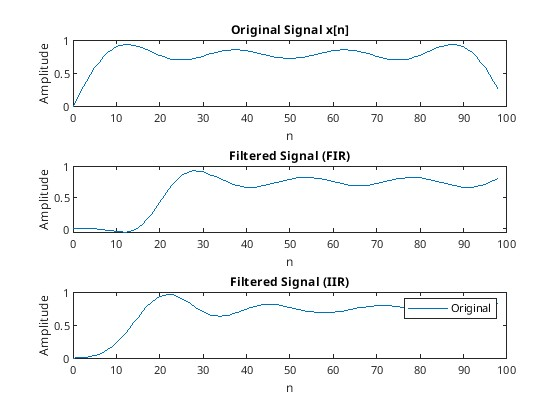
\includegraphics[width=0.8\textwidth]{../Ex01.jpg}
  \end{center}

  We can see a consistent phase shift compared to the original signal for FIR and IIR filtered signals.
  However, this phase shift seems to be more pronounced for the FIR filter, 
  the IIR filter seems to be closer to the original signal (it seems to preserver the signal better).

\end{aufgabe} \pagebreak

\begin{aufgabe}{} % Exercise 2 ---------------------------------------------------------

  We are given the difference equation 
  $$
  y[n] = x[n] - \frac{1}{15} y[n-1] + \frac25 y[n-2].
  $$

  \begin{enumerate}
    \item We sketch the corresponding block diagram:
  
    \begin{center}
      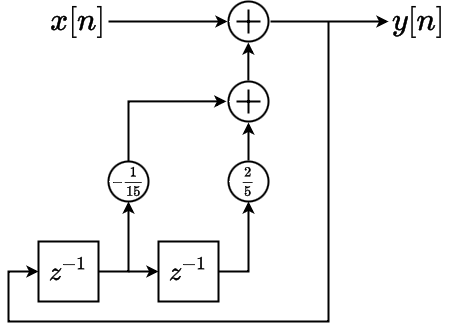
\includegraphics[width=0.4\textwidth]{../Ex02_a.png}
    \end{center}

    \item The system is an IIR Filter. This is because in the difference equation we have non-zero $a$ coefficients, i.e., it is a recursive filter.

    \item To find the transfer function, we first need to transform the system to the $z$-domain. For the transformation we use the linearity of the $z$-transformation. We assume that the signal is causal, i.e., $x[n] = y[n] = 0$ for $n < 0$.
    \begin{align}
      & y[n]
      = x[n] - \frac{1}{15} y[n-1] + \frac25 y[n-2] \\
      &\hspace*{0.6em}\rotatebox{90}{\FT} \\
      & Y(z)
      = X(z) - \frac{1}{15} z^{-1} Y(z) + \frac25 z^{z-2} Y(z)
      \quad \Longleftrightarrow \\
      & Y(z) \left( 1 + \frac{1}{15} z^{-1} - \frac25 z^{-2} \right)
      = X(z)
      \quad \Longleftrightarrow \\
      & Y(z)
      = \left( 1 + \frac{1}{15} z^{-1} - \frac25 z^{-2} \right)^{-1} X(z)
    \end{align}

    We can see that the transfer function $H(z) = \frac{Y(z)}{X(z)}$ is given by

    \begin{align}
      H(z)
      & = \left( 1 + \frac{1}{15} z^{-1} - \frac25 z^{-2} \right)^{-1} \\
      & = \frac{1}{1 + \frac{1}{15} z^{-1} - \frac25 z^{-2}} \\
      & = \frac{1}{1 + \frac{1}{15} z^{-1} - \frac25 z^{-2}} \frac{z^2}{z^2} \\
      & = \frac{z^2}{z^2 + \frac{1}{15} z - \frac25} \\
    \end{align}

    \item The roots of the numerator are clearly 0. The roots of the denominator can be determined from $z^2 + \frac{1}{15} z - \frac25 = 0$:
    \begin{align}
       z_{1,2} 
       & = - \frac{1}{30} \pm \sqrt{\frac{1}{1125} - \frac{8}{20}} \\
       & = - \frac{1}{30} \pm j \sqrt{\frac{8980}{22500}} \\
       & = - \frac{1}{30} \pm j \frac{\sqrt{8980}}{150} \\
       & \approx - 0.0333 \pm j 0.0574
    \end{align}

    You can see a sketch of the pole-zero map:
    \begin{center}
      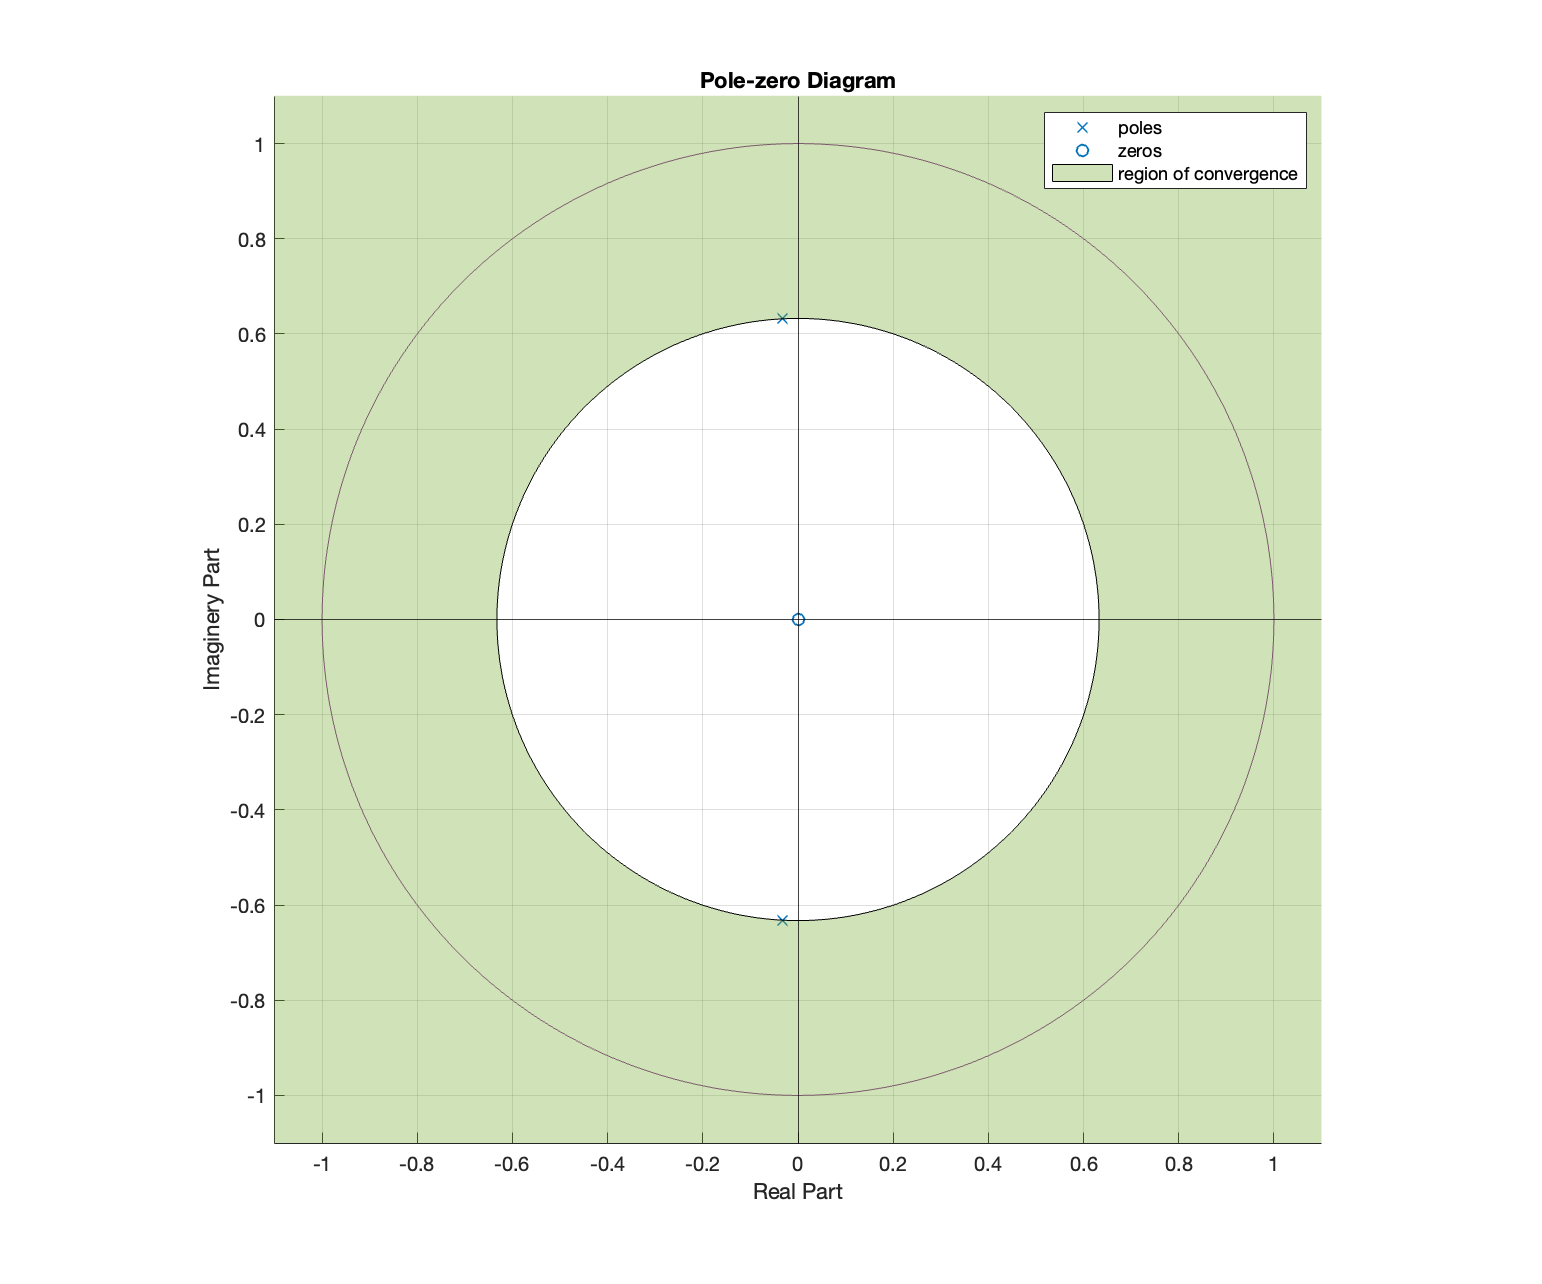
\includegraphics[width=0.8\textwidth]{../Ex02_d.png}
    \end{center}

    \item The system is stable. This can be seen by the region of convergence including the unit circle.

  \end{enumerate}

\end{aufgabe} \pagebreak


\begin{aufgabe}{} % Exercise 3 ---------------------------------------------------------

  We are given a set of poles and zeros:
  \begin{itemize}
    \item Zeros: $N_1 = -1$, $N_2 = j$, $N_3 = -j$
    \item Poles: $P_1 = 0$, $P_2 = 0.75 + j0.25$, $P_3 = 0.27 - 0.25j$
  \end{itemize}

  \begin{enumerate}
    \item This filter has only real coefficients, since when we express the transfer function in the pole-zero representation then we can see that the numerator and denominator both contain a complex number and their corresponding conjugate, meaning that when we multiply it out we will be left with only real coefficients.

    \item You can see a sketch of the pole-zero map:
    \begin{center}
      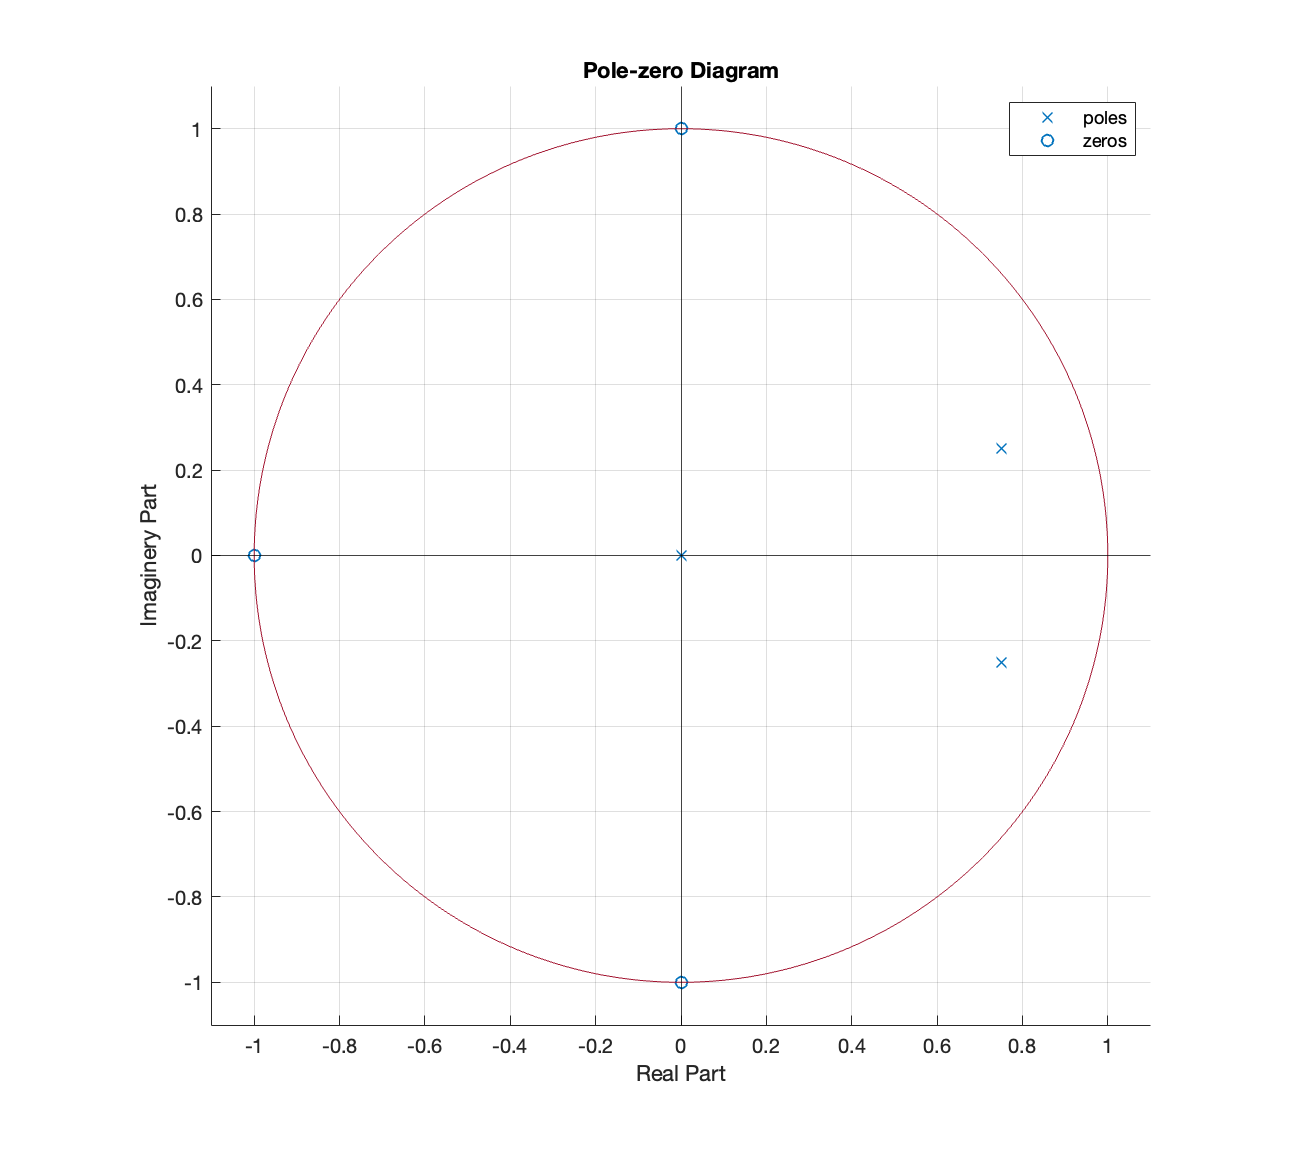
\includegraphics[width=0.8\textwidth]{../Ex03_b.png}
    \end{center}

    \item The transfer function can be obtained by writing it first in pole-zero representation and then multiplying out the clauses :
    \begin{align}
      H(z)
      &= b_0 z^{M-N} \frac{(z-N_1)(z-N_2)(z-N_3)}{(z-P_1)(z-P_2)(z-P_3)} \\
      &= b_0 \frac{(z+1)(z+j)(z-j)}{z(0.75+j0.25)(0.27-0.25j)} \\
      &= b_0 \frac{z^3 + z^2 + z + 1}{z^3 - 1.5z^2 + 0.625z} \\
      &= \frac{b_0z^3 + b_0z^2 + b_0z + b_0}{z^3 - 1.5z^2 + 0.625z} \\
      &= \frac{b_0 + b_0z^{-1} + b_0z^{-2} + b_0z^{-3}}{1 - 1.5z^{-1} + 0.625z^{-2}} \\
    \end{align}

    \item The block diagram of a direct-form-I implementation of the filter can be seen:
    \begin{center}
      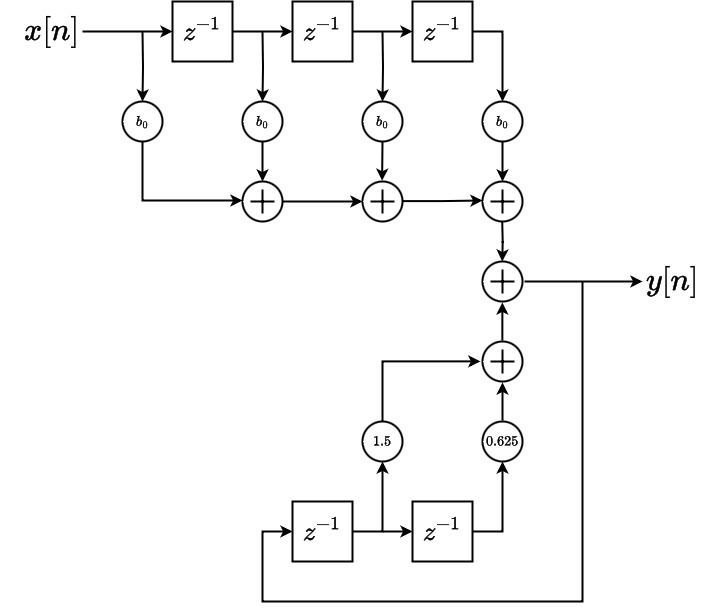
\includegraphics[width=0.6\textwidth]{../Ex03_d.png}
    \end{center}

    \item The magnitude and phase response can be seen:
    
    \begin{center}
      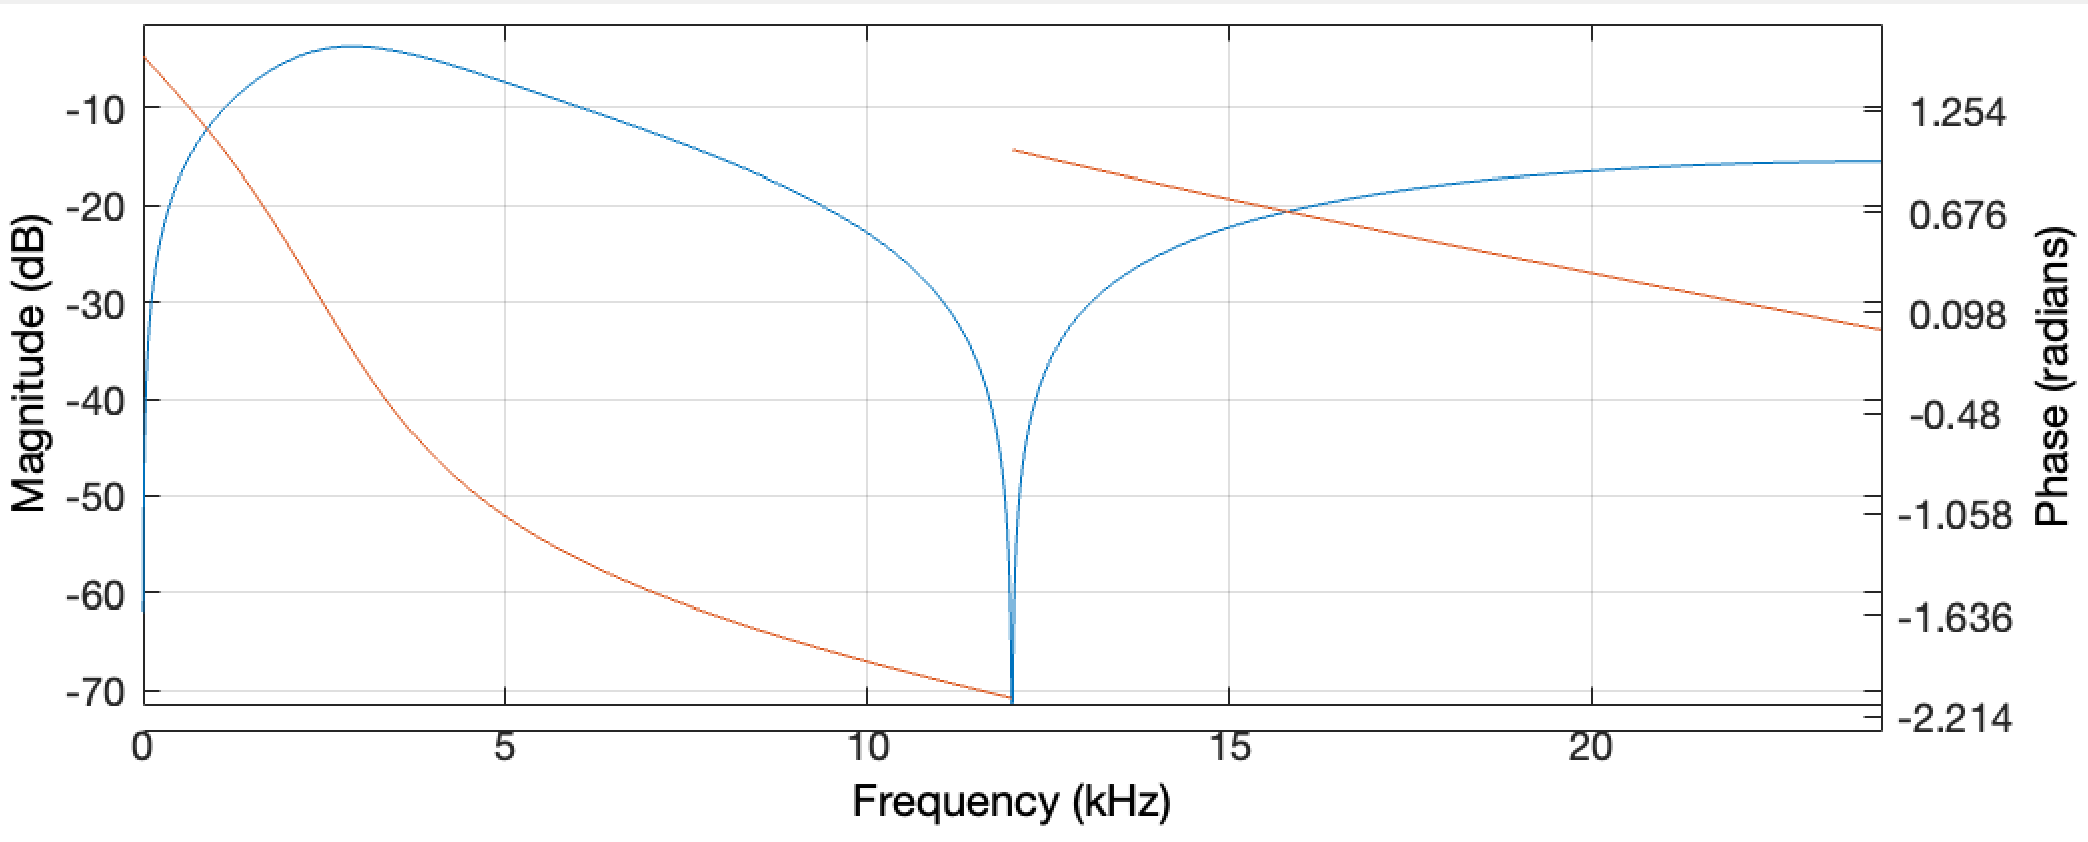
\includegraphics[width=0.8\textwidth]{../Ex03_e.png}
    \end{center}

    \item The impulse response for $0 \leq n \leq 50$ can be seen:

    \begin{center}
      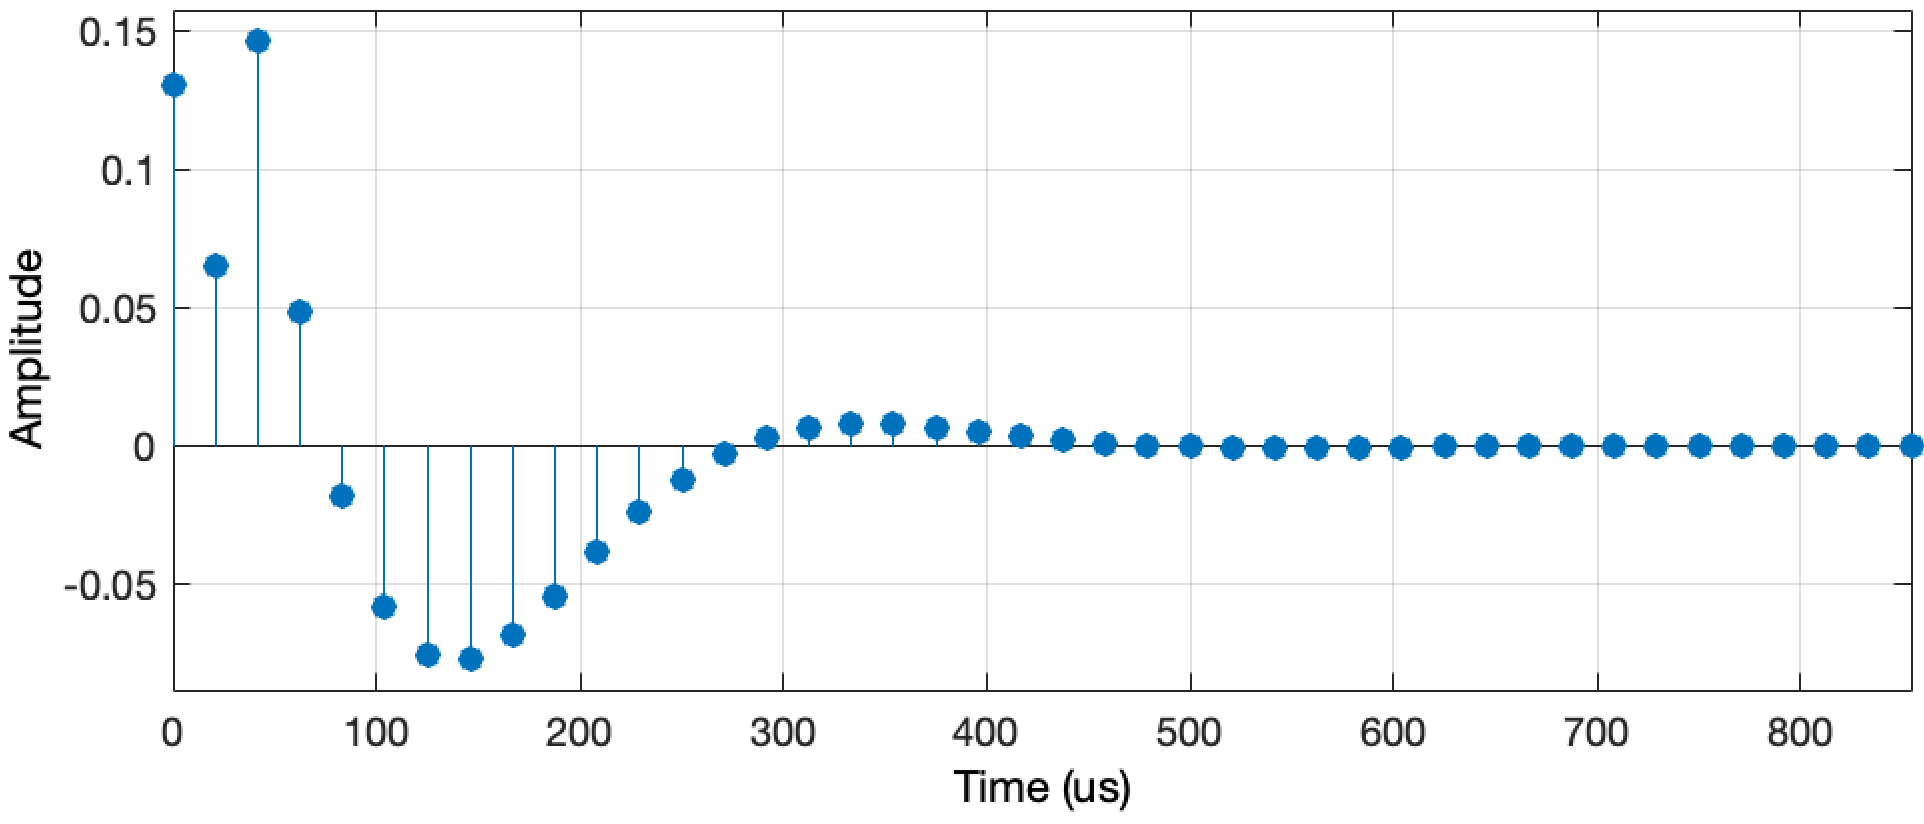
\includegraphics[width=0.8\textwidth]{../Ex03_f.png}
    \end{center}

  \end{enumerate}

\end{aufgabe} \pagebreak


\begin{aufgabe}{} % Exercise 4 ---------------------------------------------------------

An analogue signal is sampled with a sampling frequency $f_{\mathrm{s}}=20 \mathrm{kHz}$ and filtered subsequently. \\

\smallskip

The digital lowpass filter should exhibit the following specification:  \\  
- Passband cutoff frequency: $f_{\text {pass }}=3.4 \mathrm{kHz}$       \\
- Stopband cutoff frequency: $f_{\text {stop }}=4 \mathrm{kHz}$         \\
- Allowed ripple in the passband: $\pm 5 \%$                            \\
- Minimum stopband attenuation: $45 \mathrm{~dB}$

\begin{enumerate}
  \item Specify the normalized radian frequencies for the passband $\Omega_{\text {pass }}$ and the stopband $\Omega_{\text {stop }}$, the passband tolerance $\delta_1$ and the stopband tolerance $\delta_2$ \\
    
    $\Omega_{\text{pass}} = \frac{2\pi f_{\text{pass}}}{f_s} = \frac{2\pi \times 3.4 \text{kHz}}{20 \text{kHz}} \approx 1.0681$ \\
    $\Omega_{\text{stop}} = \frac{2\pi f_{\text{stop}}}{f_s} = \frac{2\pi \times 4 \text{kHz}}{20 \text{kHz}} \approx 1.2566$ \\

    \smallskip

    $\delta_1 = 0.05$ (given) \\
    $\delta_2 = 10^{-\frac{45}{20}} \approx 0.0056$
  \item What is the ideal impulse response $h_{\text {ideal }}[n]$ for the ideal frequency response
          $$
          H_{\text {ideal }}(\Omega)=\left\{\begin{array}{ll}
          1 & \text { for } 0 \leq|\Omega| \leq \Omega_0 \\
          0 & \text { for } \Omega_0 \leq|\Omega| \leq \pi
          \end{array},\right.
          $$
    $\Omega_0 = \frac{\Omega_{\text{pass}} + \Omega_{\text{stop}}}{2} = \frac{1.0681 + 1.2566}{2} \approx 1.1624$

    $h_{\text{ideal}}[n] = \frac{\Omega_0}{\pi} \operatorname{sinc}(n \Omega_0) = \frac{1.1624}{\pi} \operatorname{sinc}(n \cdot 1.1624)$

  \item Which two measures are necessary to deduce a realizable FIR system of order $N$ from the ideal impulse response $h_{\text {ideal }}[n]$ ?
          
    \smallskip
    Desired frequency response and windowing function.
  
  \item How can the decrease to the specified filter order $N$ be interpreted, and which effect on the frequency response of the realizable filter does that have?
  
  That means we are using a shorter finite impulse response (FIR) filter. \\
    For the frequency response, we get: \\
    - wider main lobes \\
    - increased side lobe levels \\
    - broader transition width \\

  \pagebreak
  \item Design an FIR filter of order $N=20$ with a rectangular window with a corner radian frequency $\Omega_0$. Plot its frequency response and the tolerance scheme in one plot.

  \begin{center}
    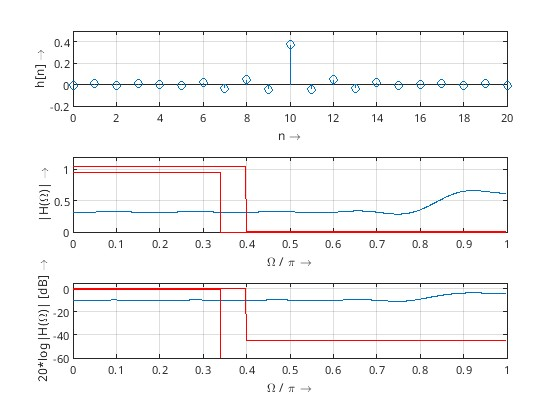
\includegraphics[width=0.8\textwidth]{../dsp_5_4.jpg}
  \end{center}

  \item Is the tolerance scheme being violated? Can the tolerance scheme be fulfilled by increasing the filter order to $N=90$ ? \\
  
    \smallskip
    Yes it exceeds the stopband tolerance, and yes we can see that this is the case below.

    \begin{center}
      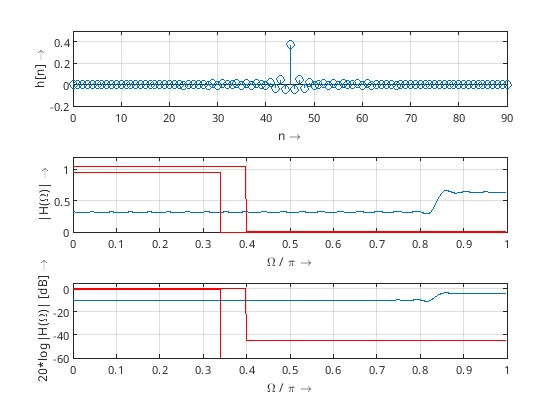
\includegraphics[width=0.8\textwidth]{../dsp_5_4-90.jpg}
    \end{center}

  \item Now, use a hamming window instead of the rectangular window (for $N=90$ ) and assess the result.
  
  \begin{center}
    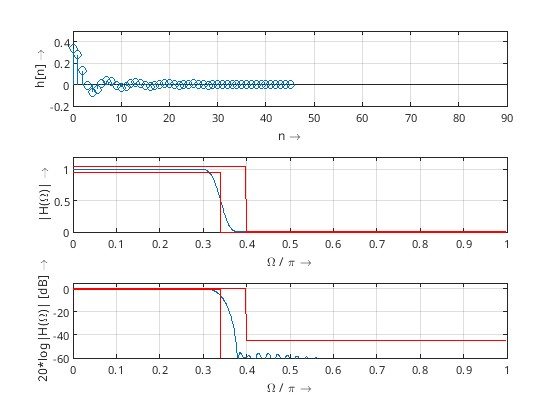
\includegraphics[width=0.8\textwidth]{../dsp_5_4_g-90.jpg}
  \end{center}

  We get a sharp transition between passband and stopband (good filter performance).

  \item se the MATLAB filterDesigner to design an elliptic IIR filter fulfilling the above described requirements. What is the order of this filter? What is the disadvantage of this filter?
    
  \begin{center}
    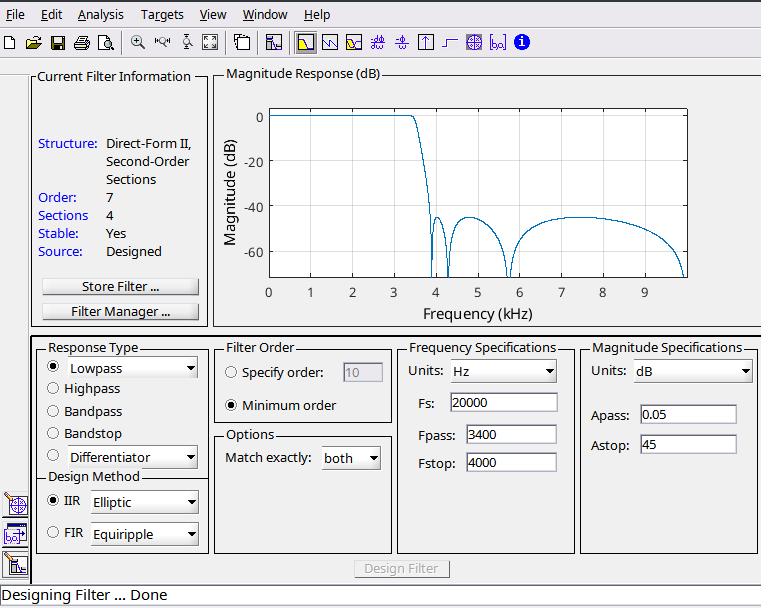
\includegraphics[width=0.7\textwidth]{../Ex04_h.png}
  \end{center}
  
  \smallskip
  
  The order is 7. Elliptic filters have ripple in both passband and stopbands.


\end{enumerate}



\end{aufgabe} \pagebreak


\end{document}
